\documentclass[]{article}
\usepackage{lmodern}
\usepackage{amssymb,amsmath}
\usepackage{ifxetex,ifluatex}
\usepackage{fixltx2e} % provides \textsubscript
\ifnum 0\ifxetex 1\fi\ifluatex 1\fi=0 % if pdftex
  \usepackage[T1]{fontenc}
  \usepackage[utf8]{inputenc}
\else % if luatex or xelatex
  \ifxetex
    \usepackage{mathspec}
  \else
    \usepackage{fontspec}
  \fi
  \defaultfontfeatures{Ligatures=TeX,Scale=MatchLowercase}
\fi
% use upquote if available, for straight quotes in verbatim environments
\IfFileExists{upquote.sty}{\usepackage{upquote}}{}
% use microtype if available
\IfFileExists{microtype.sty}{%
\usepackage{microtype}
\UseMicrotypeSet[protrusion]{basicmath} % disable protrusion for tt fonts
}{}
\usepackage[margin=1in]{geometry}
\usepackage{hyperref}
\hypersetup{unicode=true,
            pdftitle={Appendix 2: Supplemental Results},
            pdfauthor={Tim M. Szewczyk, Marek Petrik, Jenica M. Allen},
            pdfborder={0 0 0},
            breaklinks=true}
\urlstyle{same}  % don't use monospace font for urls
\usepackage{graphicx,grffile}
\makeatletter
\def\maxwidth{\ifdim\Gin@nat@width>\linewidth\linewidth\else\Gin@nat@width\fi}
\def\maxheight{\ifdim\Gin@nat@height>\textheight\textheight\else\Gin@nat@height\fi}
\makeatother
% Scale images if necessary, so that they will not overflow the page
% margins by default, and it is still possible to overwrite the defaults
% using explicit options in \includegraphics[width, height, ...]{}
\setkeys{Gin}{width=\maxwidth,height=\maxheight,keepaspectratio}
\IfFileExists{parskip.sty}{%
\usepackage{parskip}
}{% else
\setlength{\parindent}{0pt}
\setlength{\parskip}{6pt plus 2pt minus 1pt}
}
\setlength{\emergencystretch}{3em}  % prevent overfull lines
\providecommand{\tightlist}{%
  \setlength{\itemsep}{0pt}\setlength{\parskip}{0pt}}
\setcounter{secnumdepth}{5}
% Redefines (sub)paragraphs to behave more like sections
\ifx\paragraph\undefined\else
\let\oldparagraph\paragraph
\renewcommand{\paragraph}[1]{\oldparagraph{#1}\mbox{}}
\fi
\ifx\subparagraph\undefined\else
\let\oldsubparagraph\subparagraph
\renewcommand{\subparagraph}[1]{\oldsubparagraph{#1}\mbox{}}
\fi

%%% Use protect on footnotes to avoid problems with footnotes in titles
\let\rmarkdownfootnote\footnote%
\def\footnote{\protect\rmarkdownfootnote}

%%% Change title format to be more compact
\usepackage{titling}

% Create subtitle command for use in maketitle
\providecommand{\subtitle}[1]{
  \posttitle{
    \begin{center}\large#1\end{center}
    }
}

\setlength{\droptitle}{-2em}

  \title{Appendix 2: Supplemental Results}
    \pretitle{\vspace{\droptitle}\centering\huge}
  \posttitle{\par}
  \subtitle{The performance of presence-based and process-based species distribution
models}
  \author{Tim M. Szewczyk, Marek Petrik, Jenica M. Allen}
    \preauthor{\centering\large\emph}
  \postauthor{\par}
    \date{}
    \predate{}\postdate{}
  
\newcommand{\beginsupplement}{\setcounter{table}{0}  \renewcommand{\thetable}{A.\arabic{table}} \setcounter{figure}{0} \renewcommand{\thefigure}{A.\arabic{figure}}}  \usepackage{longtable}  \usepackage{caption}

\begin{document}
\maketitle

{
\setcounter{tocdepth}{1}
\tableofcontents
}
\setcounter{table}{0}  \renewcommand{\thetable}{A.\arabic{table}} \setcounter{figure}{0} \renewcommand{\thefigure}{A.\arabic{figure}}

\begin{center}\rule{0.5\linewidth}{\linethickness}\end{center}

This appendix contains supplemental tables and figures to provide
additional detail for the results, including maps of \(\lambda\) and
\(N\) for each species (true, predicted, difference), as well as figures
and a table for sensitivity and specificity with the same structures as
those for TSS in the main manuscript.

\begin{figure}
    \centering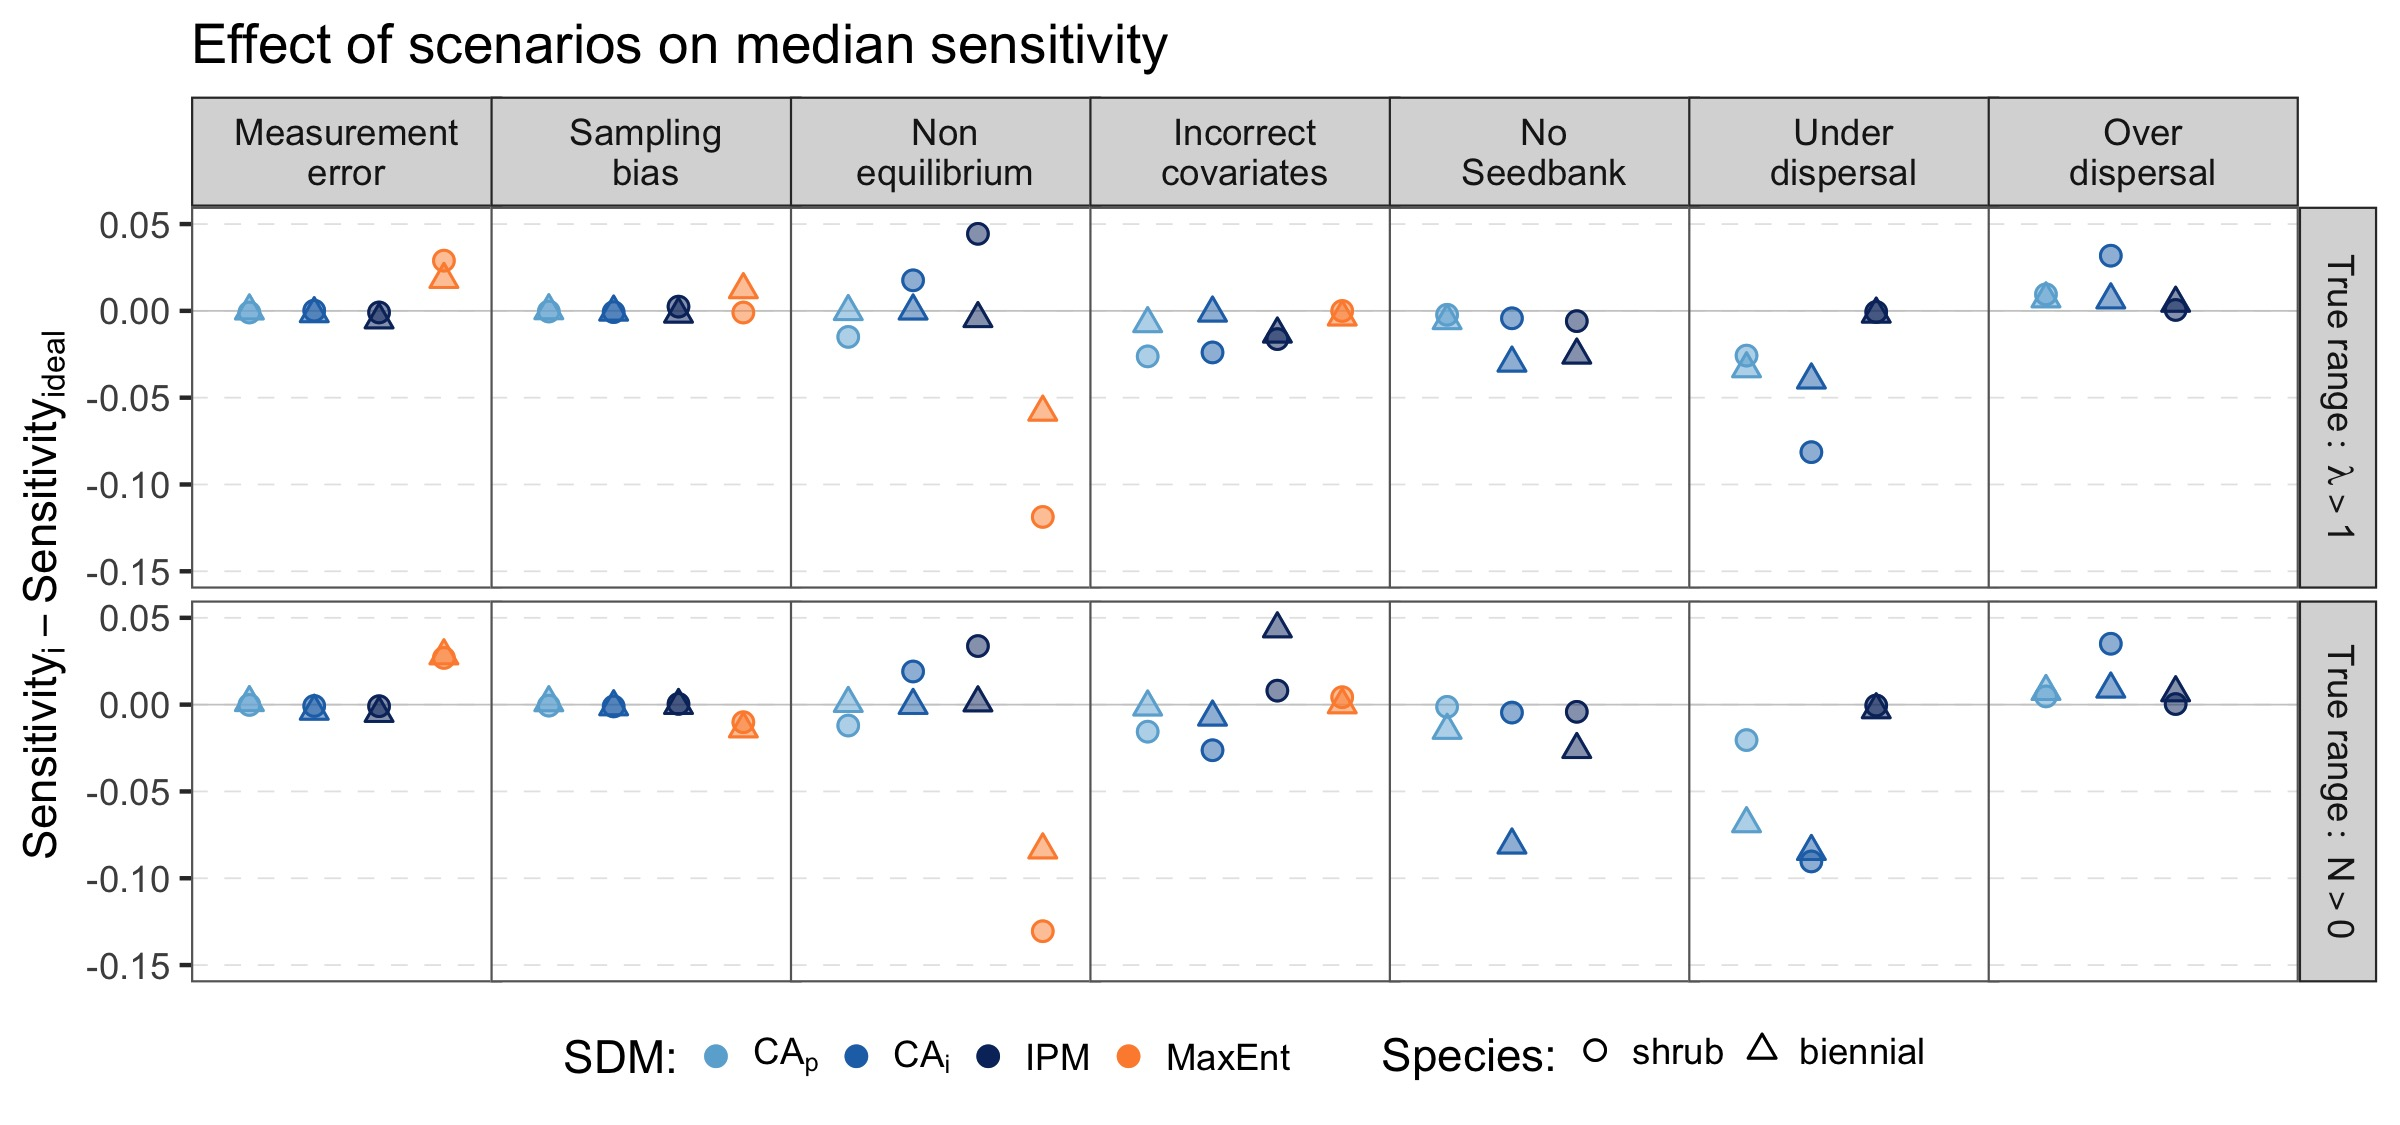
\includegraphics[width=\linewidth]{../../figs/Supp_SensvIdeal.jpg}
    \caption{\label{fig:SensitivityvIdeal} Effect of scenario on median sensitivity relative to the '\emph{ideal}' scenario. Sensitivity represents the proportion of true presences that were correctly predicted as presences.}
\end{figure}

\begin{figure}
    \centering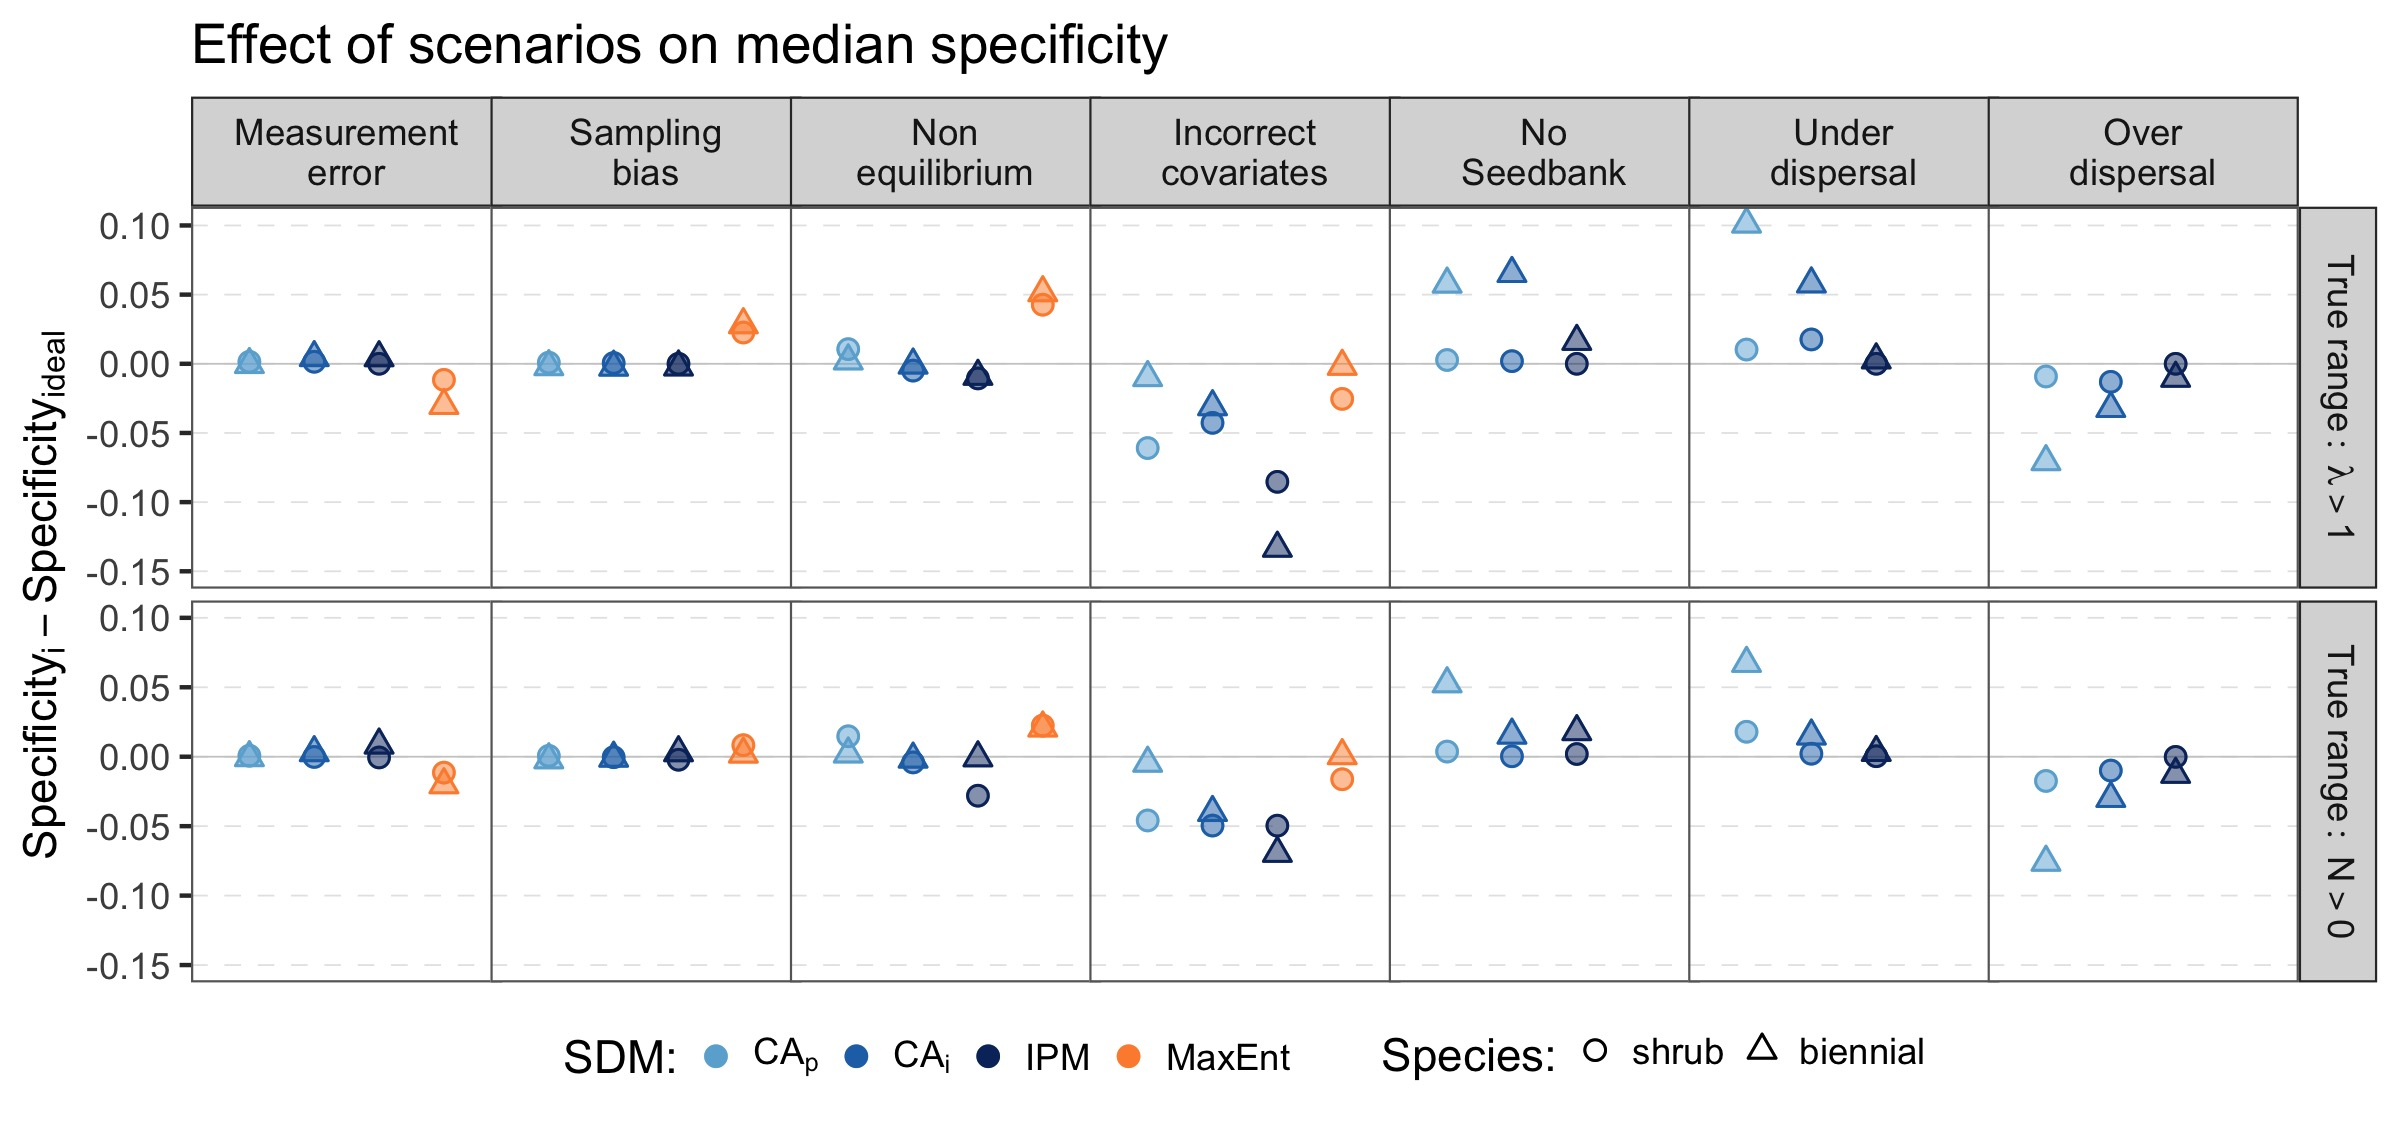
\includegraphics[width=\linewidth]{../../figs/Supp_SpecvIdeal.jpg}
    \caption{\label{fig:SpecificityvIdeal} Effect of scenario on median specificity relative to the '\emph{ideal}' scenario. Specificity represents the proportion of true absences that were correctly predicted as absences.}
\end{figure}


\end{document}
